\documentclass[11pt, oneside, a4paper]{article}
%--------This section sets up the document class and packages.
\usepackage[includeheadfoot, margin=20mm, headheight=20mm]{geometry} 
\usepackage{fancyhdr}
\usepackage{mwe}
\usepackage{amsmath}
\usepackage{amsthm}
\usepackage[utf8]{inputenc}
\usepackage{amssymb}
%\usepackage{xcolor,graphicx}
\usepackage{hyperref}
\usepackage{centernot}
\usepackage{tikz}  % Uncomment this line iff you are using the tikz package to add drawings
\usepackage{tkz-euclide}
\usepackage{pgf}
\usepackage{pgfplots}
\pgfplotsset{compat=newest}
\pgfplotsset{plot coordinates/math parser=false}
\usepackage[toc,page]{appendix}
\usepackage{hyperref}
\usepackage{pdfpages}
\usepackage{xargs}                      % Use more than one optional parameter in a new commands
%\usepackage[pdftex,dvipsnames]{xcolor}  % Coloured text etc.
% 
\usepackage[colorinlistoftodos,prependcaption]{todonotes}
\newcommandx{\unsure}[2][1=]{\todo[linecolor=red,backgroundcolor=red!25, size=\small,bordercolor=red,#1]{#2}}
\usepackage{url}
\usepackage[ruled,vlined]{algorithm2e}
\SetKwComment{Comment}{$\triangleright$\ }{}
\usepackage{listings}

\allowdisplaybreaks
\pgfplotsset{soldot/.style={color=blue,only marks,mark=*}} \pgfplotsset{holdot/.style={color=blue,fill=white,only marks,mark=*}}

\usepackage{tocloft}
\renewcommand{\cftsecleader}{\cftdotfill{\cftdotsep}}
\renewcommand\labelenumi{(\roman{enumi})}

%--- This section makes possible customized theorem numbering.
\newtheorem{innercustomgeneric}{\customgenericname}
\providecommand{\customgenericname}{}
\newcommand{\newcustomtheorem}[2]{%
  \newenvironment{#1}[1]
  {%
   \renewcommand\customgenericname{#2}%
   \renewcommand\theinnercustomgeneric{##1}%
   \innercustomgeneric
  }
  {\endinnercustomgeneric}
}
\newcustomtheorem{cthm}{Theorem}
\newcustomtheorem{caxm}{Axiom}
\newcustomtheorem{clem}{Lemma}
\newcustomtheorem{ccor}{Corollary}
\newcustomtheorem{cprop}{Proposition}
\newcustomtheorem{cdefn}{Definition}
\newcustomtheorem{ceg}{Example}
\newcustomtheorem{crmk}{Remark}
\newcustomtheorem{ccus}{}
\newcustomtheorem{cprob}{Problem}

%---The following code sets up the way theorems are typeset and labeled.
\newtheorem{thm}{Theorem}
\newtheorem{lem}[thm]{Lemma}
\newtheorem{cor}[thm]{Corollary}
\newtheorem{prop}[thm]{Proposition}
\theoremstyle{definition}
\newtheorem{defn}[thm]{Definition}
\newtheorem{axm}[thm]{Axiom}
\newtheorem{eg}[thm]{Example}
\theoremstyle{remark}
\newtheorem{rmk}[thm]{Remark}
\newtheorem{sol}{Solution}

% \numberwithin{equation}{subsection}
% \numberwithin{thm}{section}

% \newtheorem*{thm}{Theorem}
% \newtheorem*{lem}{Lemma}
% \newtheorem*{cor}{Corollary}
% \newtheorem*{prop}{Proposition}
% \theoremstyle{definition}
% \newtheorem*{defn}{Definition}
% \newtheorem*{axm}{Axiom}
% \newtheorem*{eg}{Example}
% \theoremstyle{remark}
% \newtheorem*{rmk}{Remark}
% \newtheorem*{sol}{Solution}


%---The following code defines a few extra commands that will be useful in some exercises.
\newcommand{\abs}[1]{\lvert#1\rvert}     % Absolute value symbol
\newcommand{\Abs}[1]{\Bigg\lvert#1\Bigg\rvert}     % Absolute value symbol (big)
\newcommand{\Z}{\mathbb Z}              % The set of integers
\newcommand{\Q}{\mathbb Q}              % The set of rationals
\newcommand{\R}{\mathbb R}              % The set of reals
\newcommand{\N}{\mathbb N}              % The set of natural numbers
\newcommand{\C}{\mathbb C}              % The set of complex numbers
\newcommand{\F}{\mathbb F}  

\newcommand{\ZZ}{\mathcal{Z}}
\newcommand{\OO}{\mathcal{O}}
\newcommand{\CC}{\mathcal{C}}
\newcommand{\UU}{\mathcal{U}}
\newcommand{\power}{\mathcal{P}}         % The power set of a set
\newcommand{\bfun}{\mathcal{F}}          % The finite subsets
\newcommand{\Id}{\mathrm{Id}}            % The identity function
\newcommand{\nil}{\emptyset}             % Empty set
\newcommand{\inflim}[1]{\lim_{#1\to\infty}} % Limit to infinity
\newcommand{\ninflim}[1]{\lim_{#1\to\infty}}% Limit to negative infinity
\providecommand{\BVec}[1]{\mathbf{#1}}   % Bold font for vectors
\DeclareMathOperator{\gon}{gon}          % A polygon
\DeclareMathOperator{\Fun}{Fun}          % The set of all functions from one set to another
\DeclareMathOperator{\Perm}{Perm}        % The set of all permutations on a set
\DeclareMathOperator{\Int}{int} %interior of a set
\DeclareMathOperator{\cl}{cl} %closure of a set
\DeclareMathOperator{\diam}{diam}
\DeclareMathOperator{\sinc}{sinc}
\DeclareMathOperator{\rank}{rank}
\DeclareMathOperator{\Span}{span}
\DeclareMathOperator{\len}{length}
%\newcommand{\Re}{\mathrm{Re}} %real part

\providecommand{\LIN}[1]{{\color{blue}#1}} %Linda's notes

% Dave's macros
\definecolor{colorDAS}{RGB}{255,127,0}
\providecommand{\DAS}[1]{{\color{colorDAS}#1}}     % Dave's comments

%---header/style/enumeration-------
\pagestyle{fancy}
\lhead{Capstone}
\chead{MCS}
\rhead{2018-2019 Semester 1}
\author{Linfan XIAO\\
Supervisor: Prof. David Smith}
%----------------------------------

%-----------MY INFORMATION---------
%\title{{\fontfamily{qbk}\selectfont
\title{Capstone report 2\\
Algorithmic solution of high order partial differential equations\\
in Julia via the Fokas transform method}
\date{\vspace{-5ex}}
%----------------------------------
%unnumbered sections in TOC
%\setcounter{secnumdepth}{0}

%-----This is where the GOOD STUFF begins---
\begin{document}

\maketitle

\thispagestyle{fancy}

\tableofcontents
\newpage
\section{Introduction}
\subsection{Motivation}
Evolution partial differential equations (PDEs) relate a quantity, such as temperature, to its rates of change with respect to both time (hence ``evolution'') and position. Evolution PDEs can be used to describe or model a variety of phenomena in physics, such as wave propagation and particle motion. This project concerns solving a certain class of initial-boundary value problems (IBVP) for evolution PDEs in the finite interval\cite{Smith2016} correctly and efficiently. 

To motivate the project, suppose we wish to solve some IBVPs say, to study a physics phenomenon (or produce CGI animation for a sci-fi movie that wins the Academy Award in visual effects and the Golden Raspberry Award in everything else). Certain simple IBVPs (henceforth referred to as type I problems) may be solved algorithmically via classical transform pairs such as the Fourier transform (Figure \ref{fig:classical_transform}).
\begin{figure}[htpb!]
    \centering
    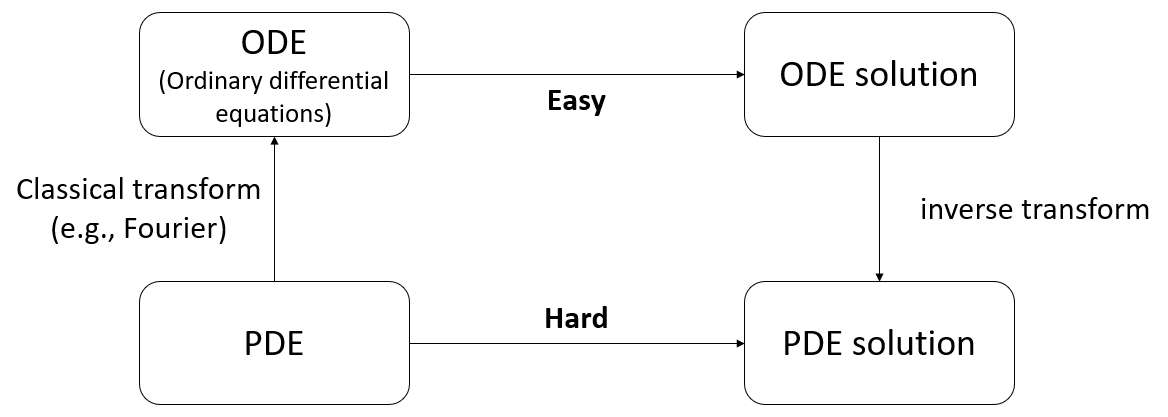
\includegraphics[width=0.8\textwidth]{classical_transform.png}
    \caption{Solving type I IBVPs using classical transform pairs.}
    \label{fig:classical_transform}
\end{figure}

For more complicated IBVPs (henceforth referred to as type II problems), however, no such classical transform pairs exist. In fact, solving these IBVPs typically requires a combination of ad-hoc methods. These methods are often specific to the given problem and cannot be generalized to problems with different parameters (e.g., IBVP involving PDE of a different order or different boundary conditions). % (Figure \ref{fig:ad-hoc_methods}).
% \begin{figure}[htpb!]
%     \centering
%     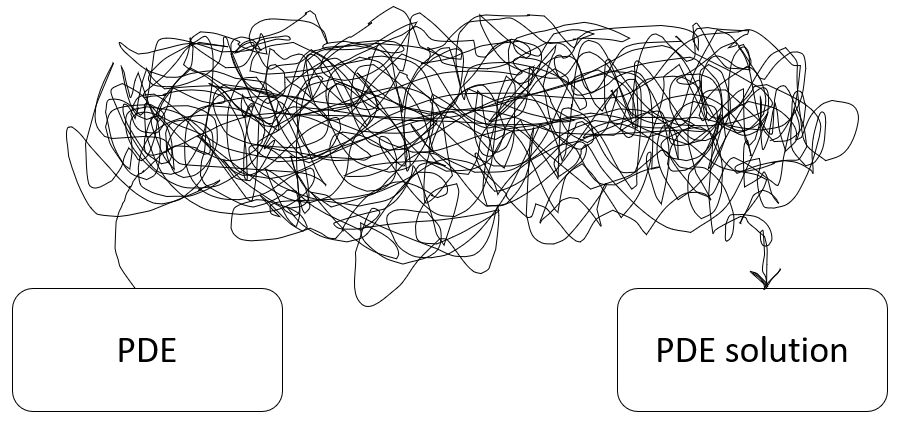
\includegraphics[width=0.65\textwidth]{ad-hoc_methods.png}
%     \caption{Solving IBVPs (type II) by finding ad-hoc methods.}
%     \label{fig:ad-hoc_methods}
% \end{figure}

The ``Fokas method''\cite{Fokas2008} extends the idea of transform pairs to solving type II problems by constructing non-classical transform pairs based on the problem parameters. Since appropriate transform pairs may now be constructed for IBVPs with different parameters, this means that the Fokas method allows solving an entire class of IBVPs algorithmically in a manner similar to Figure \ref{fig:classical_transform} (Figure \ref{fig:non-classical_transform}).
\begin{figure}[htpb!]
    \centering
    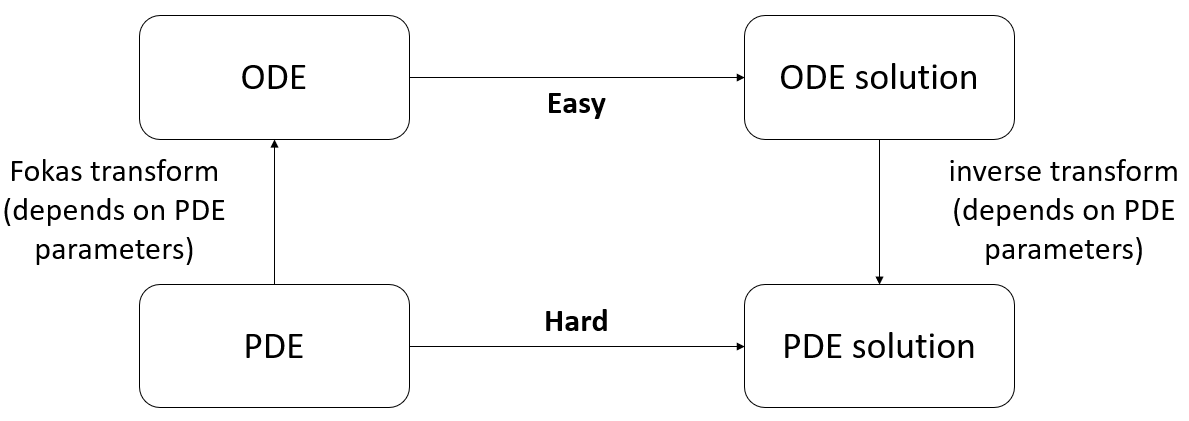
\includegraphics[width=0.8\textwidth]{non-classical_transform.png}
    \caption{Solving type II IBVPs using non-classical transform pairs.}
    \label{fig:non-classical_transform}
\end{figure}

To characterize this class of IBVPs that can be solved by the Fokas method\cite[p.9]{Smith2016}, we first define linearly independent boundary forms\footnote{These terms will be defined systematically in the report.} $B_j: C^\infty[0,1]\to \C$ (where $C^\infty[0,1]$ denotes the class of real-valued functions differentiable for all orders on $[0,1]$) by
\[B_j\phi := \sum_{k=0}^{n-1}\left(b_{jk}\phi^{(k)}(0) + \beta_{jk}\phi^{(k)}(0)\right),\, j\in\{1,2,\ldots,n\}\]
where the boundary coefficients $b_{jk}$, $\beta_{jk}\in\R$. Furthermore, define
\[\Phi:=\{\phi\in C^\infty[0,1]:\, B_j\phi = 0\,\forall j\in\{1,2,\ldots,n\}\}\]
to be the set of smooth functions $\phi$ satisfying the homogeneous boundary conditions $B_j\phi=0$ for all $j\in\{1,2,\ldots,n\}$.
Then the Fokas method allows solving any IBVP that can be written as
\begin{alignat*}{3}
    (\partial_t + aS)q(x,t) &= 0\quad &\forall (x,t)&\in (0,1)\times (0,T)\\
    q(x,0) &= q_0(x)\quad &\forall x&\in [0,1]\\
    q(\cdot, t) &\in \Phi \quad &\forall t&\in [0,T],
\end{alignat*}
where $a$ is a complex constant, $S$ is a spatial differential operator (i.e., a differential operator in the spatial variable $x$) of oder $n$, $(0,1)\times (0,T)$ is some domain, and $q_0\in \Phi$ is arbitrary. (For the IBVP to be well-posed, $a$ and $n$ need to satisfy certain constraints.) The first equation is a PDE relating a quantity $q$ to its temporal and spatial rates of change $\partial_t[q]$ and $aS[q]$, the second equation is an initial condition when the temporal variable $t=0$, and the third equation corresponds to boundary conditions as a function of the spatial variable $x$. 
% An example of this class of IBVPs is the linear Schr\"{o}dinger equation, given by
% \[ih\frac{\partial w}{\partial t} + \frac{h^2}{2m}\frac{\partial^2 w}{\partial x^2} - kxw = 0,\]
% where $w(x,t)$ is the wave function, $h$ is the Planck's constant, $m$ is the mass of the particle, and $kx$ describes the potential energy of the particle in the force field. Indeed, it can be written as
% \[(\partial_t + aS)q(x,t) = 0\]
% where $q=w$, $S = \frac{\partial^2}{\partial x^2}$, $a = \frac{h}{2mi}$, 

The Fokas method allows solving the above class of IBVPs algorithmically, i.e., it provides the correct analytic solution determinisically for any IBVP that can be written in the above form. Using the Fokas method by hand, however, is laborious. Thus, the first goal of this project is to implement the Fokas method as a Julia package that allows mathematicians to quickly obtain the analytic solutions of complicated IBVPs. We choose the Julia language for its support for high-performance scientific computing as well as its popularity among the research community due to being open-source. On the other hand, solutions of complicated IBVPs usually involve infinite sums and series, and having numerical descriptions of them would help with understanding and visualizing them. Thus, the second goal of this project is to build a analytic-numerical integrator tailored to providing accurate numerical approximations of the analytic solutions of the above IBVPs.

\subsection{Report outline}
This report focuses on the first goal of the project, i.e., implementing the Fokas method in Julia.

For appropriate transform pair $f(x)=f_x(F)$ and $F(\lambda)=F_\lambda(f)$ found using the Fokas method, the solution to the above IBVP is given by\cite[p.15]{Smith2016}
\[q(x,t) = f_x(e^{-a\lambda^n t}F_\lambda(f)).\]
Thus, the key component of the implementation is to construct the transform pairs.

The first part of the report focuses on constructing the adjoint of a given homogeneous boundary condition in preparation for finding the Fokas transform pairs. This part of the report features revisions based on the supervisor's comments on report 1. The second part of the report focuses on implementing the Fokas transform pairs, featuring progress made since report 1.

We will conclude the report with a summary of the progress so far with respect to the plan in the project proposal. This will be followed by a brief discussion of plans for the next steps.

\section{Constructing the adjoint of a homogeneous boundary condition}
Given a linear map $T$ from inner product spaces $V$ to $W$ (denoted as $T\in\mathcal{L}(V,W)$), the adjoint of $T$ is the function $T^\star:W\to V$ with
\begin{equation}\label{eq:linear map adjoint}
    \langle Tv, w\rangle = \langle v, T^\star w\rangle
\end{equation}
for $v\in V$, $w\in W$, where $\langle \cdot \rangle$ denotes inner products defined on $V$ and $W$ \cite[p.204]{Axler1997}. The ``adjoint'' mentioned in the first paragraph is an analogous notion defined for boundary value problems. The adjoint boundary condition associated with the adjoint problem relates to that of the original problem in a way that is important to making the Fokas transform pairs work as we would like them to. Thus, the first step in implementing the Fokas method is to construct the adjoint of a homogeneous boundary condition.

To this end, an algorithm to construct adjoint boundary conditions has been created. The report will focus on the algorithm's development and implementation. We begin by introducing the preliminary materials on which the algorithm depends. To make the report self-contained, referenced definitions, theorems, and proofs are included in the report, with frequent supplies of the student's own remarks and proofs so as to make the results relevant to the construction algorithm. 
%\footnote{The preliminaries section is essentially a review of the book material mixed with the student's notes, tailored to the purpose of developing the construction algorithm. Because the contents are mixed, citations in the section body are omitted and are represented by the citation in the section title. A version where the student's notes are highlighted separately is also available, if needed.}

We then present an outline of the construction algorithm, referencing definitions and theorems introduced in the preliminaries section. The outline is in higher-level, abstract form, with occasional pseudo-code illustrations when deemed necessary. 

After that, we briefly discuss the implementation of the algorithm in Julia. The discussion will focus on the characterizations of key mathematical objects, notable features, and completion status.

\subsection{Preliminaries}
\begin{defn}\cite[p.81]{CoddingtonLevinson}\label{defn:linear differential operator}
    A \textbf{linear differential operator} $L$ of order $n$ ($n>1$) on interval $[a,b]$ is defined by
    \[Lx = p_0x^{(n)} + p_1x^{(n-1)} + \cdots + p_{n-1}x' + p_nx,\]
    where the $p_k$ are complex-valued functions of class $C^{n-k}$ on $[a,b]$ and $p_0(t)\neq 0$ on $[a,b]$.
\end{defn}

\begin{defn}\cite[p.84]{CoddingtonLevinson}\label{defn:adjoint linear differential operator}
    Given a linear differential operator $L$ of order $n$ as in Definition \ref{defn:linear differential operator}, the operator $L^+$ given by
    \[L^+x = (-1)^n (\bar{p}_0 x)^{(n)} + (-1)^{n-1}(\bar{p}_1 x)^{(n-1)} +\cdots +\bar{p}_nx\]
    (where $\bar{p}_k$ is the complex conjugate of $p_k$ for $k\in\{0,\ldots,n\}$) is the \textbf{adjoint} of $L$.
\end{defn}

\begin{defn}\cite[p.284]{CoddingtonLevinson}\label{defn:homogeneous boundary conditions}
    \textbf{Homogeneous boundary conditions} refer to a set of equations of the type
    \begin{equation}\label{eq:homogeneous boundary conditions}
        \sum_{k=1}^n (M_{jk}x^{(k-1)}(a) + N_{jk}x^{(k-1)}(b))=0 \quad (j=1,\ldots,m) 
    \end{equation}
    where $M_{jk}, N_{jk}$ are complex constants.
\end{defn}

\begin{defn}\cite[p.284]{CoddingtonLevinson}\label{defn:homogeneous boundary value problem}
    A \textbf{homogeneous boundary value problem} concerns finding the solutions of 
    \[Lx=0\] on some interval $[a,b]$ which satisfy some homogeneous boundary conditions (Definition \ref{defn:homogeneous boundary conditions}).
\end{defn}

For a homogeneous boundary value problem $\pi$ with linear differential operator $L$ and some (homogeneous) boundary conditions, an adjoint problem $\pi^+$ involves the adjoint linear differential operator $L^+$ and some (homogeneous) adjoint boundary conditions. The adjoint boundary conditions are such that an equation similar to (\ref{eq:linear map adjoint}) exists for solutions of $\pi$ and those of $\pi^+$, with the inner product $(\cdot)$ defined as $(u,v) := \int_a^b u\bar{v}\,dt$ for $u, v\in C^n$ on $[a,b]$. In the following sections, we seek to characterize the adjoint boundary conditions and describe an algorithm to construct them.

The construction algorithm depends on two important results, namely Green's formula and the boundary-form formula. Generally speaking, Green's formula allows characterizing a form, which, when used in the boundary-form formula, gives rise to the desired construction. 

We begin with the Green's formula.

\subsubsection{Green's formula}
\begin{thm}\cite[p.284]{CoddingtonLevinson}{(Green's formula)}\label{thm:green's formula}
    For $u, v\in C^n$ on $[a,b]$,
    \begin{equation}\label{eq:green's formula}
        \int_{t_1}^{t_2}(Lu)\bar{v}\,dt - \int_{t_1}^{t_2}u(\overline{L^+v})\,dt = [uv](t_2) - [uv](t_1) 
    \end{equation}
    where $a\leq t_1<t_2\leq b$ and $[uv](t)$ is the form in $(u, u', \ldots, u^{(n-1)})$ and $(v, v', \ldots, v^{(n-1)})$ given by
    \begin{equation}\label{eq:[uv](t) defn}
        [uv](t)=\sum_{m=1}^n\sum_{j+k=m-1}(-1)^j u^{(k)}(t)(p_{n-m}\bar{v})^{(j)}(t)
    \end{equation}
\end{thm}
Using the form $[uv](t)$, we define an important $n\times n$ matrix $B$ whose entries $B_{jk}$ satisfy
\begin{equation}\label{eq:[uv](t) in B matrix}
    \begin{split}
        [uv](t) = \sum_{j,k=1}^n B_{jk}(t)u^{(k-1)}(t)\bar{v}^{(j-1)}(t).
    \end{split}
\end{equation}
Note that
\begin{align*}
    [uv](t) &= \sum_{m=1}^n\sum_{j+k=m-1}(-1)^j u^{(k)}(t)(p_{n-m}\bar{v})^{(j)}(t)\\
        &= \sum_{m=1}^n\sum_{j+k=m-1}(-1)^j u^{(k)}(t)\left(\sum_{\ell=0}^j\binom{j}{\ell}p_{n-m}^{(j-\ell)}(t)\bar{v}^{(\ell)}(t)\right)\\
        &= \sum_{m=1}^n\sum_{k=0}^{m-1}(-1)^{m-1-k} u^{(k)}(t)\left(\sum_{\ell=0}^{m-1-k}\binom{m-1-k}{\ell}p_{n-m}^{(m-1-k-\ell)}(t)\bar{v}^{(\ell)}(t)\right)\\
        &= \sum_{m=1}^n\sum_{k=1}^{m}(-1)^{m-k}\left(\sum_{\ell=0}^{m-k}\binom{m-k}{\ell}p_{n-m}^{(m-k-\ell)}(t)\bar{v}^{(\ell)}(t)\right)u^{(k-1)}(t)\quad\mbox{(shifting $k$ to $k+1$)}\\
        &= \sum_{k=1}^n\sum_{m=k}^n (-1)^{m-k}\left(\sum_{\ell=0}^{m-k}\binom{m-k}{\ell}p_{n-m}^{(m-k-\ell)}(t)\bar{v}^{(\ell)}(t)\right)u^{(k-1)}(t).
\end{align*}

To find $B_{jk}$, we need to extract the coefficients of $u^{(k-1)}\bar{v}^{(j-1)}$. We first note that, fixing $m$ and $k$, when $\ell=j-1$, the coefficient of $\bar{v}^{(j-1)}$ is
\begin{align*}
    \binom{m-k}{j-1}p_{n-m}^{(m-k-j+1)}(t).
\end{align*}
To find the coefficient of $u^{(k-1)}\bar{v}^{(j-1)}$, we need to fix $k$ and collect the above coefficient across all values of $m$. Since $m$ goes up to $n$, $m-k$ goes up to $n-k$. Since $\ell\leq m-k$, $\ell=j-1$ implies $j-1\leq m-k$. Thus, $m-k$ ranges from $j-1$ to $n-k$. Let $\ell':=m-k$, then $m=k+\ell'$, and the above equation becomes
\begin{align*}
    [uv](t) 
    &= \sum_{k=1}^n\sum_{j=1}^n (-1)^{\ell'}\left(\sum_{\ell'=j-1}^{n-k}\binom{\ell'}{j-1}p_{n-(k+\ell')}^{(\ell'-(j-1))}(t)\right)\bar{v}^{(j-1)}(t)u^{(k-1)}(t)\\
    &= \sum_{j,k=1}^n \left(\sum_{\ell=j-1}^{n-k}\binom{\ell}{j-1}p^{(\ell-j+1)}_{n-k-\ell}(t)(-1)^\ell\right)u^{(k-1)}(t)\bar{v}^{(j-1)}(t)\quad\mbox{(replace $\ell'$ by $l$)}.
\end{align*}
Thus,
\[B_{jk}(t) = \sum_{\ell=j-1}^{n-k}\binom{\ell}{j-1}p^{(\ell-j+1)}_{n-k-\ell}(t)(-1)^\ell.\]
We note that for $j+k>n+1$, or $j-1>n-k$, $l$ is undefined. This means that terms $u^{(k-1)}(t)\bar{v}^{(j-1)}(t)$ with $j+k>n+1$ does not exist in $[uv](t)$. Thus, $B_{jk}(t)=0$. Also, for $j+k=n+1$, or $j-1=n-k$,
\[B_{jk}(t) = \binom{j-1}{j-1}p^{(j-1-j+1)}_{j-1-(j-1)}(t)(-1)^{j-1} = (-1)^{j-1}p_0(t).\] 
Thus, the matrix $B$ has the form
\begin{equation}\label{eq:B(t)}
    B(t)=\begin{bmatrix}
        B_{11} & B_{12} & \cdots & \cdots & B_{1\,n-1} & p_0(t)\\
        B_{21} & B_{22} & \cdots & \cdots & -p_0(t) & 0\\
        \vdots & \vdots & \ddots &  & \vdots & \vdots\\
        \vdots & \vdots &  & \ddots & \vdots & \vdots\\
        (-1)^{n-1}p_0(t) & 0 & \cdots & \cdots & 0 & 0
    \end{bmatrix}.
\end{equation}
We note that because $p_0(t)\neq 0$ on $[a,b]$ (as required in Definition \ref{defn:linear differential operator}), $B(t)$ is square with $\det B(t)=(p_0(t))^n\neq 0$ on $[a,b]$. Thus, $B(t)$ is nonsingular for $t\in [a,b]$.


Now we seek another matrix $\hat{B}$ that embodies both the characteristics of $B$ and those of the interval $[a,b]$. This concerns writing the right-hand side of Green's formula in matrix form. We begin by introducing the following definitions.

\begin{defn}\cite[p.285]{CoddingtonLevinson}\label{defn:f cdot g}
    For vectors $f=(f_1,\ldots,f_k)$, $g=(g_1,\ldots,g_k)$, define the product
    \[f\cdot g:=\sum_{i=1}^k f_i\bar{g}_i.\]
    Note that $f\cdot g = g^*f$ where $^*$ denotes conjugate transpose.
\end{defn}

\begin{defn}\cite[p.285]{CoddingtonLevinson}\label{defn:semibilinear form}
    A \textbf{semibilinear form} is a complex-valued function $\mathcal{S}$ defined for pairs of vectors $f=(f_1,\ldots,f_k)$, $g=(g_1,\ldots,g_k)$ satisfying
    \begin{align*}
        \mathcal{S}(\alpha f+\beta g, h)&=\alpha\mathcal{S}(f,h) + \beta\mathcal{S}(g,h)\\
        \mathcal{S}(f, \alpha g + \beta h) &= \bar{\alpha}\mathcal{S}(f,g) + \bar{\beta}\mathcal{S}(f, h)
    \end{align*}
    for any complex numbers $\alpha, \beta$ and vectors $f,g,h$.
\end{defn}
We note that if
\[S = \begin{bmatrix}
    s_{11} & \cdots & s_{1k}\\
    \vdots &  & \vdots\\
    s_{k1} & \cdots & s_{kk}
\end{bmatrix},\]
then $Sf\cdot g$ is given by
\begin{equation}\label{eq:semibilinear form}
    \begin{split}
    \mathcal{S}(f,g) &:= Sf\cdot g = \begin{bmatrix}
        s_{11} & \cdots & s_{1k}\\
        \vdots & & \vdots\\
        s_{k1} & \cdots & s_{kk}
    \end{bmatrix} \begin{bmatrix}
        f_1\\
        \vdots\\
        f_k
    \end{bmatrix} \cdot \begin{bmatrix}
        g_1\\
        \vdots\\
        g_k
    \end{bmatrix} = \begin{bmatrix}
        \sum_{j=1}^k s_{1j}f_j\\
        \vdots\\
        \sum_{j=1}^k s_{kj}f_j
    \end{bmatrix}\cdot \begin{bmatrix}
        g_1\\
        \vdots\\
        g_k
    \end{bmatrix}\\
    &= \sum_{i=1}^k\left(\sum_{j=1}^k s_{ij}f_j\right)\bar{g}_i =\sum_{i,j=1}^k s_{ij}f_i\bar{g}_i.
    \end{split}
\end{equation}
To see that this is a semibilinear form:
\begin{align*}
    \mathcal{S}(\alpha f+\beta g, h)
    &= \sum_{i,j=1}^k s_{ij}(\alpha f_j + \beta g_j)\bar{h}_i
    = \alpha \sum_{i,j=1}^k s_{ij}f_j\bar{h}_i + \beta \sum_{i,j=1}^k g_j\bar{h}_i\\
    &= \alpha Sf\cdot h + \beta Sg\cdot h
    = \alpha\mathcal{S}(f,h) + \beta\mathcal{S}(g,h);
\end{align*}
and similarly,
\begin{align*}
    \mathcal{S}(f, \alpha g + \beta h)
    &= \sum_{i,j=1}^k s_{ij}f_j(\overline{\alpha g_i + \beta h_i})
    = \bar{\alpha}\sum_{i,j=1}^k s_{ij}f_j\bar{g}_i + \bar{\beta}\sum_{i,j=1}^k f_j \bar{h}_i\\
    &= \bar{\alpha}Sf\cdot g + \bar{\beta}Sf\cdot h
    = \bar{\alpha}\mathcal{S}(f,g) + \bar{\beta}\mathcal{S}(f,h).
\end{align*}

Under a similar matrix framework, we see that $[uv](t)$ is a semibilinear form with matrix $B(t)$: Let $\vec{u}=(u, u', \ldots, u^{(n-1)})$ and $\vec{v}=(v, v', \ldots, v^{(n-1)})$. Then we have
\begin{equation}\label{[uv](t) in semibilinear form}
    \begin{split}
    [uv](t) &= \sum_{j,k=1}^n B_{jk}(t)u^{(k-1)}(t)\bar{v}^{(j-1)}(t)\quad\mbox{(by \eqref{eq:[uv](t) in B matrix})}\\
    &= \sum_{i,j=1}^n (B_{ij}u^{(j-1)}\overline{v}^{(i-1)})(t)\\
    &= (B\vec{u}\cdot \vec{v})(t)\quad\mbox{(by (\ref{eq:semibilinear form}))}\\
    &=: \mathcal{S}(\vec{u},\vec{v})(t).
    \end{split}
\end{equation}
With this notation, we can rewrite the right-hand side of Green's formula as a semibilinear form below:
\begin{equation}\label{eq:green's formula in semibilinear form}
    \begin{split}
    [uv](t_2)-[uv](t_1) &= \sum_{j,k=1}^n B_{jk}(t_2)u^{(k-1)}(t_2)\bar{v}^{(j-1)}(t_2) - \sum_{j,k=1}^n B_{jk}(t_2)u^{(k-1)}(t_1)\bar{v}^{(j-1)}(t_1)\\
    &= B(t_2)\vec{u}(t_2)\cdot \vec{v}(t_2) - B(t_1)\vec{u}(t_1)\cdot \vec{v}(t_1)\\
    &= \begin{bmatrix}
        B_{11}(t_2) & \cdots & B_{1n}(t_2)\\
        \vdots &  & \vdots\\
        B_{n1}(t_2) & \ldots & B_{nn}(t_2)
    \end{bmatrix} 
    \begin{bmatrix}
    u(t_2)\\
    \vdots\\
    u^{(n-1)}(t_2)
    \end{bmatrix}\cdot 
    \begin{bmatrix}
        \bar{v}(t_2)\\
        \vdots\\
        \bar{v}^{(n-1)}(t_2)
    \end{bmatrix} -\\
    &\qquad \begin{bmatrix}
        B_{11}(t_1) & \cdots & B_{1n}(t_1)\\
        \vdots &  & \vdots\\
        B_{n1}(t_1) & \ldots & B_{nn}(t_1)
    \end{bmatrix} 
    \begin{bmatrix}
    u(t_1)\\
    \vdots\\
    u^{(n-1)}(t_1)
    \end{bmatrix}\cdot 
    \begin{bmatrix}
        \bar{v}(t_1)\\
        \vdots\\
        \bar{v}^{(n-1)}(t_1)
    \end{bmatrix}\\
    &= \begin{bmatrix}
        -B_{11}(t_1) & \cdots & -B_{1n}(t_1)\\
        \vdots &  & \vdots\\
        -B_{n1}(t_1) & \ldots & -B_{nn}(t_1)
    \end{bmatrix} 
    \begin{bmatrix}
    u(t_1)\\
    \vdots\\
    u^{(n-1)}(t_1)
    \end{bmatrix}\cdot 
    \begin{bmatrix}
        \bar{v}(t_1)\\
        \vdots\\
        \bar{v}^{(n-1)}(t_1)
    \end{bmatrix} + \\
    &\qquad \begin{bmatrix}
        B_{11}(t_2) & \cdots & B_{1n}(t_2)\\
        \vdots &  & \vdots\\
        B_{n1}(t_2) & \ldots & B_{nn}(t_2)
    \end{bmatrix} 
    \begin{bmatrix}
    u(t_2)\\
    \vdots\\
    u^{(n-1)}(t_2)
    \end{bmatrix}\cdot 
    \begin{bmatrix}
        \bar{v}(t_2)\\
        \vdots\\
        \bar{v}^{(n-1)}(t_2)
    \end{bmatrix}\\
    &= \begin{bmatrix}
        -B_{11}(t_1) & \cdots & -B_{1n}(t_1) & 0 & \cdots & 0\\
        \vdots &  & \vdots & \vdots &  & \vdots\\
        -B_{n1}(t_1) & \cdots & -B_{nn}(t_1) & 0 & \cdots & 0\\
        0 & \cdots & 0 & B_{11}(t_2) & \cdots & B_{1n}(t_2)\\
        \vdots &  & \vdots & \vdots &  & \vdots\\
        0 & \cdots & 0 & B_{n1}(t_2) & \cdots & B_{nn}(t_2)
    \end{bmatrix} 
    \begin{bmatrix}
        u(t_1)\\
        \vdots\\
        u^{(n-1)}(t_1)\\
        u(t_2)\\
        \vdots\\
        u^{(n-1)}(t_2)
    \end{bmatrix}\cdot
    \begin{bmatrix}
        \bar{v}(t_1)\\
        \vdots\\
        \bar{v}^{(n-1)}(t_1)\\
        \bar{v}(t_2)\\
        \vdots\\
        \bar{v}^{(n-1)}(t_2)
    \end{bmatrix}\\
    &= \begin{bmatrix}
        -B(t_1) & 0_n\\
        0_n & B(t_2)
    \end{bmatrix}
    \begin{bmatrix}
        u(t_1)\\
        \vdots\\
        u^{(n-1)}(t_1)\\
        u(t_2)\\
        \vdots\\
        u^{(n-1)}(t_2)
    \end{bmatrix}\cdot
    \begin{bmatrix}
        \bar{v}(t_1)\\
        \vdots\\
        \bar{v}^{(n-1)}(t_1)\\
        \bar{v}(t_2)\\
        \vdots\\
        \bar{v}^{(n-1)}(t_2)
    \end{bmatrix}\\
    &=:\hat{B}
    \begin{bmatrix}
        \vec{u}(t_1)\\
        \vec{u}(t_2)
    \end{bmatrix}\cdot
    \begin{bmatrix}
        \vec{v}(t_1)\\
        \vec{v}(t_2)
    \end{bmatrix}.
\end{split}
\end{equation}
Recall that $\det(\lambda A) = \lambda^n\det(A)$ for $n\times n$ matrix $A$. Thus,
\[\det\hat{B}= \det(-B(t_1))\det(B(t_2))= (-1)^n\det B(t_1)\det B(t_2)\]
since $B(t_1)$ is $n\times n$. Since $B(t)$ is nonsingular for $t\in [a,b]$ (as shown before), $\hat{B}$ is nonsingular for $t_1, t_2\in [a,b]$.

To recapitulate, given a linear differential operator $L$ which involves functions $p_0,\ldots,p_n$ and an interval $[a,b]$, from the Green's formula, we have defined a matrix $B$ which depends on $p_0,\ldots,p_n$ and a matrix $\hat{B}$ which depends on $B$ and $[a,b]$. These objects will be important in constructing an adjoint boundary condition using the boundary-form formula, which we now turn to.

\subsubsection{Boundary-form formula}
Before introducing the boundary-form formula, we need a set of definitions and results concerning boundary conditions.

\begin{defn}\cite[p.286]{CoddingtonLevinson}\label{defn:boundary form}
    Given any set of $2mn$ complex constants $M_{ij}, N_{ij}$ ($i=1,\ldots, m;\,j=1,\ldots,n$), define $m$ \textbf{boundary operators (boundary forms)} $U_1,\ldots,U_m$ for functions $x$ on $[a,b]$, for which $x^{(j)}$ ($j=1,\ldots,n-1$) exists at $a$ and $b$, by
    \begin{equation}\label{eq:U_i defn}
        U_i x = \sum_{j=1}^n (M_{ij}x^{(j-1)}(a) + N_{ij}x^{(j-1)}(b))\quad\mbox{($i=1,\ldots,m$)} 
    \end{equation}
    $U_i$ are \textbf{linearly independent} if the only set of complex constants $c_1, \ldots, c_m$ for which
    \[\sum_{i=1}^m c_i U_ix=0\]
    for all $x\in C^{n-1}$ on $[a,b]$ is $c_1=c_2=\cdots =c_m=0$.
\end{defn}

\begin{defn}\cite[p.286]{CoddingtonLevinson}\label{defn:vectory boundary form}
    A \textbf{vectory boundary form} $U=(U_1,\ldots,U_m)$ is a vector whose components are boundary forms (Definition \ref{defn:boundary form}). When $U_1,\ldots,U_m$ are linearly independent, we say that $U$ has rank $m$. We assume $U$ has full rank below.
\end{defn}

With the above definitions, we can now write a set of homogeneous boundary conditions (Definition \ref{defn:homogeneous boundary conditions}) in matrix form. Define
\[
    \xi:= \begin{bmatrix}x\\ x'\\ \vdots \\ x^{(n-1)}
    \end{bmatrix};
        \quad
    U := \begin{bmatrix}U_1\\ U_2\\ \vdots \\ U_m
    \end{bmatrix};
        \quad
    M := \begin{bmatrix}
        M_{11} & \cdots & M_{1n}\\
        \vdots &  & \vdots\\
        M_{m1} & \cdots & M_{mn}
    \end{bmatrix};
    \quad
    N := \begin{bmatrix}
        N_{11} & \cdots & N_{1n}\\
        \vdots &  & \vdots\\
        N_{m1} & \cdots & N_{mn}
    \end{bmatrix}.
\]
Then the set of homogeneous boundary conditions in (\ref{eq:homogeneous boundary conditions}) can be written as
\[Ux = M\xi(a) + N\xi(b).\]
Indeed:
\begin{align*}
    M\xi(a) + N\xi(b) &= \begin{bmatrix}
        M_{11} & \cdots & M_{1n}\\
        \vdots &  & \vdots\\
        M_{m1} & \cdots & M_{mn}
    \end{bmatrix}\begin{bmatrix}x(a)\\ x'(a)\\ \vdots \\ x^{(n-1)}(a)
        \end{bmatrix} + \begin{bmatrix}
            N_{11} & \cdots & N_{1n}\\
            \vdots &  & \vdots\\
            N_{m1} & \cdots & N_{mn}
        \end{bmatrix}\begin{bmatrix}x(b)\\ x'(b)\\ \vdots \\ x^{(n-1)}(b)
        \end{bmatrix}\\
        &= \begin{bmatrix}
            \sum_{j=1}^n M_{1j}x^{(j-1)}(a)\\
            \vdots\\
            \sum_{j=1}^n M_{mj}x^{(j-1)}(a)
        \end{bmatrix} + \begin{bmatrix}
            \sum_{j=1}^n N_{1j}x^{(j-1)}(b)\\
            \vdots\\
            \sum_{j=1}^n N_{mj}x^{(j-1)}(b)
        \end{bmatrix}\\
        &= \begin{bmatrix}
            \sum_{j=1}^n (M_{1j}x^{(j-1)}(a) + N_{1j}x^{(j-1)}(b))\\
            \vdots\\
            \sum_{j=1}^n (M_{mj}x^{(j-1)}(a) + N_{mj}x^{(j-1)}(b))
        \end{bmatrix}\\
        &= \begin{bmatrix}
            U_1 x\\
            \vdots\\
            U_m x
        \end{bmatrix} = \begin{bmatrix}U_1\\ U_2\\ \vdots \\ U_m
        \end{bmatrix}x = Ux.
\end{align*}
Based on the above, we propose another way to write $U_x$. Define the $m\times 2n$ matrix
\[(M:N):=\begin{bmatrix}
    M_{11} & \cdots & M_{1n} & N_{11} & \cdots & N_{1n}\\
    \vdots &  & \vdots & \vdots & & \vdots\\
    M_{m1} & \cdots & M_{mn} & N_{m1} & \cdots & N_{mn}
\end{bmatrix}.\]
Then $U_1,\ldots,U_m$ are linearly independent if and only if $\rank(M:N)=m$, or equivalently, $\rank(U)=m$. 
%Recall that the rank of a matrix is the largest number of linearly independent rows or columns in it. For a matrix $A_{m\times n}$, $\rank(A)\leq \min\{m,n\}$ and $\rank(A)=\rank(A^T)$.
Moreover, $Ux$ can also be written as
\begin{align*}
    Ux &= \begin{bmatrix}
        \sum_{j=1}^n (M_{1j}x^{(j-1)}(a) + N_{1j}x^{(j-1)}(b))\\
        \vdots\\
        \sum_{j=1}^n (M_{mj}x^{(j-1)}(a) + N_{mj}x^{(j-1)}(b))
    \end{bmatrix}\\
    &= \begin{bmatrix}
        M_{11} & \cdots & M_{1n} & N_{11} & \cdots & N_{1n}\\
        \vdots &  & \vdots & \vdots & & \vdots\\
        M_{m1} & \cdots & M_{mn} & N_{m1} & \cdots & N_{mn}
    \end{bmatrix} \begin{bmatrix}x(a)\\\vdots\\x^{(n-1)}(a)\\ x(b)\\\vdots\\x^{(n-1)}(b)\end{bmatrix}\\
    &= (M:N)\begin{bmatrix}
        \xi(a)\\
        \xi(b)
    \end{bmatrix}.
\end{align*}

Having proposed a compact way to represent a set of homogeneous boundary conditions, we begin building our way to characterizing the notion of adjoint boundary condition. First, we need the notion of a complementary boundary form.

\begin{defn}\cite[p.287]{CoddingtonLevinson}\label{defn:complementary boundary form}
    If $U=(U_1,\ldots, U_m)$ is any boundary form with $\rank(U)=m$ and $U_c=(U_{m+1},\ldots,U_{2n})$ is any form with $\rank(U_c)=2n-m$ such that $(U_1,\ldots, U_{2n})$ has rank $2n$, then $U$ and $U_c$ are \textbf{complementary boundary forms}. 
    
    Note that extending $U_{1},\ldots, U_{m}$ to $U_1,\ldots,U_{2n}$ is equivalent to embedding the matrix $(M:N)$ in a $2n\times 2n$ nonsingular matrix (recall that a square matrix is nonsingular if and only if it has full rank).
\end{defn}

The characterization of adjoint boundary conditions is given by the boundary-form formula. The boundary-form formula is motivated by writing the right-hand side of Green's formula \eqref{eq:green's formula} as the linear combination of a boundary form $U$ and a complementary form $U_c$. Before finally getting to it, we need the following propositions.

\begin{prop}\cite[p.287]{CoddingtonLevinson}
    In the context of the semibilinear form \eqref{eq:semibilinear form}, we have
    \begin{equation}\label{eq:semibilinear adjoint}
        Sf\cdot g = f\cdot S^*g, 
    \end{equation}
    where $S^*$ is the conjugate transpose of $S$.
\end{prop}
\begin{proof}
    \begin{align*}
        Sf\cdot g &= \sum_{i,j=1}^k s_{ij}f_j\bar{g}_i \quad\mbox{(by \eqref{eq:semibilinear form})};\\
        f\cdot S^*g &= \begin{bmatrix}
            f_1\\
            \vdots\\
            f_k
        \end{bmatrix}\cdot \begin{bmatrix}
            \bar{s}_{11} & \cdots & \bar{s}_{k1}\\
            \vdots & & \vdots\\
            \bar{s}_{1k} & \cdots & \bar{s}_{kk}
        \end{bmatrix} \begin{bmatrix}
            g_1\\
            \vdots\\
            g_k
        \end{bmatrix}\\
        &= \begin{bmatrix}
            f_1\\
            \vdots\\
            f_k
        \end{bmatrix}\cdot \begin{bmatrix}
            \sum_{j=1}^k \bar{s}_{j1}g_j\\
            \vdots\\
            \sum_{j=1}^k \bar{s}_{jk}g_j
        \end{bmatrix}\\
        &= \sum_{i=1}^k f_i\cdot \left(\overline{\sum_{j=1}^k\bar{s}_{ji}g_j}\right)\\
        &= \sum_{i=1}^k f_i\cdot \left(\sum_{j=1}^k s_{ji}\bar{g}_j\right)\\
        &= \sum_{i,j=1}^k s_{ji}f_i\bar{g}_j = Sf\cdot g.\qedhere
    \end{align*}
\end{proof}

\begin{prop}\cite[p.287]{CoddingtonLevinson}\label{prop:unique nonsingular G in semibilinear form}
    Let $\mathcal{S}$ be the semibilinear form associated with a nonsingular matrix $S$. Suppose $\bar{f}:=Ff$ where $F$ is a nonsingular matrix. Then there exists a unique nonsingular matrix $G$ such that if $\bar{g}=Gg$, then $\mathcal{S}(f,g)=\bar{f}\cdot \bar{g}$ for all $f, g$.
\end{prop}
\begin{proof}
    Let $G:=(SF^{-1})^*$, then
    \begin{align*}
        \mathcal{S}(f,g) &= Sf\cdot g\\
        &= S(F^{-1}F)f\cdot g\\
        &= SF^{-1}(Ff)\cdot g\\
        &= SF^{-1}\bar{f} \cdot g\\
        &= \bar{f}\cdot (SF^{-1})^*g \quad\mbox{(by \eqref{eq:semibilinear adjoint})}\\
        &= \bar{f}\cdot G*g\\
        &= \bar{f}\cdot \bar{g}.
    \end{align*}
    To see that $G$ is nonsingular, note that $\det G = \det((\overline{SF^{-1}})^T) = \det(\overline{SF^{-1}}) = \overline{\det(SF^{-1})} = \overline{\det(S)\det(F)^{-1}}\neq 0$ since $S, F$ are nonsingular.
\end{proof}

\begin{prop}\cite[p.287]{CoddingtonLevinson}\label{prop:last k-j components linear combination}
    Suppose $\mathcal{S}$ is associated with the unit matrix $E$, i.e., $\mathcal{S}(f,g)=f\cdot g$. Let $F$ be a nonsingular matrix such that the first $j$ ($1\leq j<k$) components of $\bar{f}=Ff$ are the same as those of $f$. Then the unique nonsingular matrix $G$ such that $\bar{g}=Gg$ and $\bar{f}\cdot \bar{g}=f\cdot g$ (as in Proposition \ref{prop:unique nonsingular G in semibilinear form}) is such that the last $k-j$ components of $\bar{g}$ are linear combinations of the last $k-j$ components of $g$ with nonsingular coefficient matrix.
\end{prop}
\begin{proof}
    We note that for the condition on $F$ to hold, $F$ must have the form
\[\begin{bmatrix}E_j & 0_+\\
F_+ & F_{k-j}\end{bmatrix}_{k\times k}\]
where $E_j$ is the $j\times j$ identity matrix, $0_+$ is the $j\times (k-j)$ zero matrix, $F_+$ is a $(k-j)\times j$ matrix, and $F_{k-j}$ a $(k-j)\times (k-j)$ matrix. Let $G$ be the unique nonsingular matrix in Proposition \ref{prop:unique nonsingular G in semibilinear form}. Write $G$ as
\[\begin{bmatrix}G_j & G_-\\
G_= & G_{k-j}\end{bmatrix}_{k\times k}\]
where $G_j, G_-, G_=, G_{k-j}$ are $j\times j, j\times (k-j), (k-j)\times j, (k-j)\times (k-j)$ matrices, respectively. By the definition of $G$,
\[f\cdot g = Ff\cdot Gg = \bar{f}\cdot Gg = G^*\bar{f}\cdot g = G^*Ff\cdot g,\]
(where the third equality follows from a reverse application of \eqref{eq:semibilinear adjoint} with $\bar{f}$ as $f$, $G^*$ as $S$) which implies
\[G^*F = E_k.\]
Since
\begin{align*}
    G^*F &= \begin{bmatrix}
        G^*_j & G^*_=\\
        G^*_- & G^*_{k-j}
    \end{bmatrix}\begin{bmatrix}E_j & 0_+\\
    F_+ & F_{k-j}\end{bmatrix}\\
    &= \begin{bmatrix}
        G^*_j + G^*_= F_+ & G^*_= F_{k-j}\\
        G^*_- + G^*_{k-j} F_+ & G^*_{k-j}F_{k-j}
    \end{bmatrix}\\
    &= \begin{bmatrix}
        E_j & 0_{j\times (k-j)}\\
        0_{(k-j)\times j} & E_{k-j}
    \end{bmatrix}.
\end{align*}
Thus, $G^*_=F_{k-j}=0_+$, the $j\times (k-j)$ zero matrix. But $\det F = \det(E_j)\cdot \det(F_{k-j})\neq 0$, so $\det F_{k-j}\neq 0$ and we must have $G^*_==0_+$, i.e., $G_= =0_{(k-j)\times j}$. Thus, $G$ is upper-triangular, and so $\det G = \det G_j \cdot \det G_{k-j}\neq 0$, which implies $\det G_{k-j}\neq 0$ and $G_{k-j}$ is nonsingular. Hence,
\[\bar{g} = Gg = \begin{bmatrix}G_j & G_-\\
0_{(k-j)\times j} & G_{k-j}\end{bmatrix} \begin{bmatrix}
g_1\\
\vdots\\
g_k
\end{bmatrix}\]
where $G_{k-j}$ is the nonsingular coefficient matrix such that
\[\begin{bmatrix}
    \bar{g}_{j-1}\\
    \vdots\\
    \bar{g}_{k}
\end{bmatrix} = G_{k-j}\begin{bmatrix}
    g_{j-1}\\
    \vdots\\
    g_{k}
\end{bmatrix}.\]
\end{proof}

We are finally ready to introduce the boundary-form formula, the theorem central to the construction of adjoint boundary condition.

\begin{thm}\cite[p.288]{CoddingtonLevinson}{(Boundary-form formula)}\label{thm:boundary form formula}
    Given any boundary form $U$ of rank $m$ (Definition \ref{defn:boundary form}), and any complementary form $U_c$ (Definition \ref{defn:complementary boundary form}), there exist unique boundary forms $U_c^+$, $U^+$ of rank $m$ and $2n-m$, respectively, such that
    \begin{equation}\label{eq:boundary form formula}
        [xy](b)-[xy](a) = Ux\cdot U_c^+y + U_{c}x\cdot U^+y.
    \end{equation}
    If $\tilde{U}_c$ is any other complementary form to $U$, and $\tilde{U}^+_c, \tilde{U}^+$ the corresponding forms of rank $m$ and $2n-m$, then
    \begin{equation}\label{eq:adjoint boundary forms unique only up to linear transformation}
        \tilde{U}^+ y = C^*U^+y
    \end{equation}
    for some nonsingular matrix $C$.
\end{thm}
\begin{rmk}
    $U^+$ is the key object which will be defined later as an adjoint boundary condition to $U$.

    Note that the existence of $[xy](t)$ implies that a linear differential operator is involved (see (\ref{eq:[uv](t) defn})). The matrices $\hat{B}$ and $B$ in the proof also depend on this linear differential operator.

    Also note that the second statement in the theorem reflects the fact that adjoint boundary conditions are unique only up to linear transformation. This is why when the need for rigor is greater than that for convenience, we take care to use ``an'' instead of ``the'' in referring to adjoint boundary condition.
\end{rmk}
\begin{proof}
    Recall from \eqref{eq:green's formula in semibilinear form} that the left-hand side of \eqref{eq:boundary form formula} can be considered as a semibilinear form $\mathcal{S}(f,g)=\hat{B}f\cdot g$ for vectors
    \[
        f=
        \begin{bmatrix}
            x(a)\\
            \vdots\\
            x^{(n-1)}(a)\\
            x(b)\\
            \vdots\\
            x^{(n-1)}(b)
        \end{bmatrix},\,
        g=
        \begin{bmatrix}
            y(a)\\
            \vdots\\
            y^{(n-1)}(a)\\
            y(b)\\
            \vdots\\
            y^{(n-1)}(b)
        \end{bmatrix}
    \]
    with the nonsingular matrix
    \[
        \hat{B}=
        \begin{bmatrix}
            -B(a) & 0_n\\
            0_n & B(b)
        \end{bmatrix},
    \]
    where $B$ is as in (\ref{eq:B(t)}).
    Recall from a previous discussion that 
    \[Ux = M\xi(a) + N\xi(b) = (M:N)\begin{bmatrix}\xi(a)\\ \xi(b)\end{bmatrix}\]
    for $M, N, \xi$ are as defined there. With the definition of $f$, we have $f=\begin{bmatrix}\xi(a)\\ \xi(b)\end{bmatrix}$ and thus
    \[Ux = (M:N)f.\]
    By Definition \ref{defn:complementary boundary form}, $U_c x = (\tilde{M}:\tilde{N})f$ for two appropriate matrices $\tilde{M}, \tilde{N}$ for which
    \[H = \begin{bmatrix}M & N\\
    \tilde{M} & \tilde{N}\end{bmatrix}_{2n\times 2n}\]
    has rank $2n$. Thus,
    \[\begin{bmatrix}Ux\\ U_cx\end{bmatrix} = \begin{bmatrix}(M:N)f\\(\tilde{M}:\tilde{N})f\end{bmatrix} = \begin{bmatrix}M & N\\
    \tilde{M} & \tilde{N}\end{bmatrix}f = Hf.\]
    By Proposition \ref{prop:unique nonsingular G in semibilinear form}, there exists a unique $2n\times 2n$ nonsingular matrix $J$ (in fact, with $S = \hat{B}$, $F=H$, $J=G$, and $G=(SF^{-1})^\star$ where $^\star$ denotes the conjugate transpose, we have $J=(\hat{B}H^{-1})^\star$) such that $\mathcal{S}(f,g) = Hf\cdot Jg$. Let $U^+, U_c^+$ be such that
    \[Jg = \begin{bmatrix}U_c^+ y\\ U^+y\end{bmatrix},\]
    then 
    \[[xy](b)-[xy](a)=\mathcal{S}(f,g) = Hf\cdot Jg = \begin{bmatrix}Ux\\ U_cx\end{bmatrix}\cdot\begin{bmatrix}U_c^+ y \\ U^+y\end{bmatrix} = Ux\cdot U_c^+y + U_cx\cdot U^+y.\]
    Thus, \eqref{eq:boundary form formula} holds.

    The second statement in the theorem follows from Proposition \ref{prop:last k-j components linear combination} with $Hf$ and $Jg$ corresponding to $f$ and $g$.
\end{proof}

\subsubsection{Homogeneous boundary value problem and its adjoint}
With the boundary-form formula, we are now able to fully characterize the notion of ``adjoint'' for boundary value problems. In this section, we begin by defining adjoint boundary condition and adjoint boundary value problem. We then explore some properties of these adjoints as relevant to the construction algorithm.

\begin{defn}\cite[p.288-89]{CoddingtonLevinson}\label{defn:adjoint boundary condition}
    For any boundary form $U$ of rank $m$ there is associated the homogeneous boundary condition
    \begin{equation}\label{eq:homogeneous boundary condition}
        Ux=0
    \end{equation}
    for functions $x\in C^{n-1}$ on $[a,b]$. If $U^+$ is any boundary form of rank $2n-m$ determined as in Theorem \ref{thm:boundary form formula}, then the homogeneous boundary condition
    \begin{equation}\label{eq:adjoint boundary condition}
        U^+x=0
    \end{equation}
    is an \textbf{adjoint boundary condition} to (\ref{eq:homogeneous boundary condition}).
\end{defn}

Putting together $L, L^+$ and $U, U^+$, we have the definition of adjoint boundary value problem.

\begin{defn}\cite[p.291]{CoddingtonLevinson}\label{defn:adjoint boundary value problem}
    If $U$ is a boundary form of rank $m$, the problem of finding solutions of
    \[\pi_m:\,Lx=0\quad Ux=0\]
    on $[a,b]$ is a \textbf{homogeneous boundary value problem of rank $m$}. The problem
    \[\pi_{2n-m}^+:\,L^+x=0\quad U^+x=0\]
    on $[a,b]$ is the \textbf{adjoint boundary value problem to $\pi_m$}.
\end{defn}

In connection with the notion of adjoint problem introduced after Definition \ref{defn:homogeneous boundary value problem}, we now have the following property of the adjoint analogous to (\ref{eq:linear map adjoint}).

\begin{prop}\label{prop:(Lu,v)=(u,L^+v)}
    By Green's formula \eqref{eq:green's formula} and the boundary-form formula \eqref{eq:boundary form formula}, 
    \[(Lu, v) = (u, L^+v)\]
    for all $u\in C^n$ on $[a,b]$ satisfying \eqref{eq:homogeneous boundary condition} and all $v\in C^n$ on $[a,b]$ satisfying \eqref{eq:adjoint boundary condition}.
\end{prop}
\begin{proof}
    \begin{equation}
        \begin{split}
            (Lu, v) - (u, L^+v) &= \int_a^b Lu\bar{v}\,dt - \int_a^b u(\overline{L^+v})\,dt\\
            &= [uv](a) - [uv](b) \quad\mbox{(by Green's formula \eqref{eq:green's formula})}\\
            &= Uu\cdot U_c^+ v + U_c u\cdot U^+v \quad\mbox{(by boundary-form formula \eqref{eq:boundary form formula})}\\
            &= 0\cdot U_c^+ v + U_c u \cdot 0 \quad\mbox{(by \eqref{eq:homogeneous boundary condition} and \eqref{eq:adjoint boundary condition})}\\
            &= 0.\qedhere
        \end{split}
    \end{equation}
\end{proof}

In some cases, the above result is treated as the definition of the adjoint problem. Here, we treat it as a property of the adjoint after defining $L^+$ and constructing $U^+$. Yet we can still appreciate the motivation behind defining the notion of adjoint for boundary value problems.

Now, we turn to one last result that would help us in the last step of the construction algorithm, namely checking whether an adjoint boundary condition is valid.

Just like how $U$ is associated with two $m\times n$ matrices $M, N$, $U^+$ is associated with two $n\times (2n-m)$ matrices $P, Q$ such that $(P^*:Q^*)$ has rank $2n-m$ and
\begin{equation}\label{eq:U^+x in P* Q*}
    U^+x = P^*\xi(a) + Q^*\xi(b).
\end{equation}
% Note that embedding $M, N, P^*, Q^*$ in the same matrix gives
% \begin{align*}
%     \begin{bmatrix}
%         (M:N)_{m\times 2n}\\
%         (P^*:Q^*)_{(2n-m)\times 2n}
%     \end{bmatrix}_{2n\times 2n} & = \begin{bmatrix}
%         M & N\\
%         P^* & Q^*
%     \end{bmatrix},
% \end{align*}
% which is a $2n\times 2n$ matrix of full rank.
The following theorem is motivated by characterizing the adjoint condition \eqref{eq:adjoint boundary condition} in terms of the matrices $M, N, P, Q$. For our purpose, it provides a way to check whether the adjoint boundary condition found by the algorithm is indeed valid using the matrices $M, N, P, Q$.

\begin{thm}\cite[p.289]{CoddingtonLevinson}\label{thm:condition iff adjoint}
    The boundary condition $U^+x=0$ is adjoint to $Ux=0$ if and only if
    \begin{equation}\label{eq:condition iff adjoint}
        MB^{-1}(a)P = NB^{-1}(b)Q
    \end{equation}
    where $B(t)$ is the $n\times n$ matrix associated with the form $[xy](t)$ (\ref{eq:B(t)}).
\end{thm}
\begin{proof}
    Let $\eta := (y, y', \ldots, y^{(n-1)})$,
    then $[xy](t)=B(t)\xi(t)\cdot \eta(t)$ by \eqref{[uv](t) in semibilinear form}.

    Suppose $U^+x=0$ is adjoint to $Ux=0$. By definition of adjoint boundary condition (\ref{eq:adjoint boundary condition}), $U^+$ is determined as in Theorem \ref{thm:boundary form formula}. But by Theorem \ref{thm:boundary form formula}, in determining $U^+$, there exist boundary forms $U_c$, $U_c^+$ of rank $2n-m$ and $m$, respectively, such that (\ref{eq:boundary form formula}) holds. 

    Put
    \begin{align*}
        U_cx &= M_c\xi(a) + N_c\xi(b)\quad \rank(M_c:N_c) = 2n-m\\
        U_c^+y &= P_c^*\eta(a) + Q_c^*\eta(b)\quad\rank(P_c^*:Q_c^*)=m.
    \end{align*}
    Then by the boundary-form formula (\ref{eq:boundary form formula}),
    \begin{align*}
        B(b)\xi(b)\cdot \eta(b) - B(a)\xi(a)\cdot \eta(a) &= (M\xi(a) + N\xi(b))\cdot (P_c^*\eta(a) + Q_c^*\eta(b)) + \\
        &\qquad (M_c\xi(a) + N_c\xi(b))\cdot (P^*\eta(a) + Q^*\eta(b)).
    \end{align*}
    By (\ref{eq:semibilinear adjoint}), 
    \[M\xi(a)\cdot P_c^*\eta(a) = P_cM\xi(a)\cdot \eta(a).\]
    Thus,
    \begin{align*}
        B(b)\xi(b)\cdot \eta(b) - B(a)\xi(a)\cdot \eta(a) &= (P_c M + PM_c)\xi(a)\cdot \eta(a) + (Q_cM + QM_c)\xi(a)\cdot \eta(b) \\
        &\qquad (P_cN + PN_c) \xi(b)\cdot \eta(a) + (Q_cN + QN_c) \xi(b)\cdot \eta(b).
    \end{align*}
    Thus, we have
    \begin{align*}
        P_cM + PM_c &= - B(a) & P_cN + PN_c &= 0_n\\
        Q_cM + QM_c &= 0_n & Q_cN + QN_c &= B(b).
    \end{align*}
    Since $\det B(t)\neq 0$ on $t\in[a,b]$, $B^{-1}(a)$, $B^{-1}(b)$ exist, and thus
    \begin{align*}
        \begin{bmatrix}
            -B^{-1}(a)P_c & -B^{-1}(a)P\\
            B^{-1}(b)Q_c & B^{-1}(b)Q
        \end{bmatrix}
        \begin{bmatrix}
            M & N\\
            M_c & N_c
        \end{bmatrix}
        =
        \begin{bmatrix}
            E_n & 0_n\\
            0_n & E_n
        \end{bmatrix}.
    \end{align*}
    Recall that $\begin{bmatrix}
        M & N\\
        M_c & N_c
    \end{bmatrix}$ has full rank, which means that it is nonsingular (Definition \ref{defn:complementary boundary form}). Thus, the two matrices on the left are inverses of each other. So we also have
    \begin{align*}
        \begin{bmatrix}
            M & N\\
            M_c & N_c
        \end{bmatrix}
        \begin{bmatrix}
            -B^{-1}(a)P_c & -B^{-1}(a)P\\
            B^{-1}(b)Q_c & B^{-1}(b)Q
        \end{bmatrix}
        =
        \begin{bmatrix}
            E_m & 0_+\\
            0_- & E_{2n-m}
        \end{bmatrix}.
    \end{align*}
    Therefore,
    \[-MB^{-1}(a)P + NB^{-1}(b)Q = 0_+,\]
    which is \eqref{eq:condition iff adjoint}.

    Conversely, let $U_1^+$ be a boundary form of rank $2n-m$ such that
    \[U_1^+y = P_1^*\eta(a) + Q_1^*\eta(b)\]
    for appropriate $P_1^*$, $Q_1^*$ with $\rank(P_1^*:Q_1^*)=2n-m$. Suppose
    \begin{equation}\label{eq:condition iff adjoint converse}
        MB^{-1}(a)P_1 = NB^{-1}(b)Q_1
    \end{equation}
    holds.

    By the fundamental theorem of linear maps \cite[p.63]{Axler1997}, if $V$ is finite-dimensional and $T\in\mathcal{L}(V, W)$, then $\dim\ker T = \dim V - \dim \range T$. Suppose $A$ is a $n\times k$ matrix, then $A\in\mathcal{L}(\R^n, \R^k)$. Thus, in a homogeneous system of linear equations $Ax=0$, we have $\dim \ker A = \dim A - \dim \range A$. That is, the dimension of solution space $\ker A$ is the difference between the number of unknown variables and the rank of the coefficient matrix, or $\dim\range A$. Therefore, letting $u$ be a $2n\times 1$ vector, there exist exactly $2n-m$ linearly independent solutions of the homogeneous linear system $(M:N)_{m\times 2n}u=0$. By \eqref{eq:condition iff adjoint converse},
    \[MB^{-1}(a)P_1 - NB^{-1}(b)Q=0,\]
    and thus
    \[(M:N)_{m\times 2n}\begin{bmatrix}
        B^{-1}(a)P_1\\
        -B^{-1}(b)Q_1
    \end{bmatrix}_{2n\times (2n-m)} = 0_{m\times (2n-m)}.\]
    So the $2n-m$ columns of the matrix
    \[H_1:= \begin{bmatrix}
        B^{-1}(a)P_1\\
        -B^{-1}(b)Q_1
    \end{bmatrix}\]
    are solutions of this system. Since $\rank(P_1^*:Q_1^*)=2n-m$,
    \[\rank\begin{bmatrix}P_1\\ Q_1\end{bmatrix}=2n-m.\]
    Since $B(a)$, $B(b)$ are nonsingular, $\rank(H_1)=2n-m$.

    If $U^+x=P^*\xi(a) + Q^*\xi(b)=0$ is a boundary condition adjoint to $Ux=0$, then the matrix
    \[\begin{bmatrix}
        -B^{-1}(a)P_c & -B^{-1}(a)P\\
        B^{-1}(b)Q_c & B^{-1}(b)Q
    \end{bmatrix}_{2n\times 2n}\]
is nonsingular (because it has inverse $\begin{bmatrix}M & N\\ M_c & N_c\end{bmatrix}$), i.e., it has full rank. Thus, if 
    \[H = \begin{bmatrix}
        -B^{-1}(a)P\\
        B^{-1}(b)Q
    \end{bmatrix}_{n\times (2n-m)},\]
    then $\rank(H)=2n-m$. Therefore, by \eqref{eq:condition iff adjoint}, the $2n-m$ columns of $H$ also form $2n-m$ linearly independent solutions of $(M:N)u=0$, as in the case of $H_1$. Hence, there exists a nonsingular $(2n-m)\times (2n-m)$ matrix $A$ such that $H_1=HA$ (change of basis in the solution space). 
    Thus we have
    \begin{align*}
        \begin{bmatrix}
            B^{-1}(a)P_1\\
            -B^{-1}(b)Q_1
        \end{bmatrix} = H_1 = HA = \begin{bmatrix}
            B^{-1}(a)PA\\
            -B^{-1}(b)QA
        \end{bmatrix},
    \end{align*}
    or $P_1=PA$, $Q_1=QA$. Thus, 
    \[U_1^+y = P_1^*\eta(a) + Q_1^*\eta(b) = A^*P^*\eta(a) + A^*Q^*\eta(b)= A^* U^+y.\]
    Since $A^\star$ is a linear map, $U^+y=0$ implies $U_1^+y=A^*U^+y=0$. Since $A^\star$ is nonsingular, $A^{\star^{-1}}$ is also a linear map, and $A^{\star^{-1}}U_1^+y = U^+y$. Thus, $U_1^+y=0$ implies $U^+y=A^{\star^{-1}}U_1^+y=0$. Therefore, $U^+y=0$ if and only if $U_1^+y=0$. Since $U^+y=0$ is adjoint to $Ux=0$, $U_1^+y=0$ is adjoint to $Ux=0$.
\end{proof}

To recapitulate, the boundary-form formula (Theorem \ref{thm:boundary form formula}) gives us the existence and construction of adjoint boundary condition, and Theorem \ref{thm:condition iff adjoint} gives us a way to check whether a proposed adjoint boundary condition is valid. Now, we are ready to propose a construction algorithm.

\subsection{Algorithm outline}
Suppose we are given a homogeneous boundary value problem on $[a,b]$,
\[Lx=0\quad Ux=0,\]
where $L$ is a linear differential operator with order $n$ (Definition \ref{defn:linear differential operator}) and $U$ is a vector boundary form $U=(U_1,\ldots, U_n)$ (Definition \ref{defn:vectory boundary form}). (For the purpose of the project, we are only interested in cases where $m=n$.) We seek to construct a valid adjoint boundary condition $U^+x=0$ (Definition \ref{defn:adjoint boundary condition}). 

\subsubsection{Check input}
We first check that $U_1,\ldots, U_n$ are linearly independent. As noted in a previous discussion, write
\[Ux = M\xi(a) + N\xi(b),\]
then it suffices to check whether $\rank(M:N)=n$. $U$ would be considered an invalid input if $\rank(M:N)\neq n$.

\subsubsection{Find $U^+$}
Recall from Definition \ref{defn:complementary boundary form} that extending $U_1,\ldots,U_n$ to $U_1,\ldots,U_{2n}$ (where $(U_{n+1},\ldots, U_{2n})$ is a complementary boundary form $U_c$) is equivalent to embedding $(M:N)$ in a $2n\times 2n$ nonsingular matrix (where the newly added rows constitute $(\tilde{M}, \tilde{N})$ associated with $U_c$). We construct this $2n\times 2n$ nonsingular matrix from the identity matrix $E_{2n}$ and $(M:N)$ as follows. We append the rows of $E_{2n}$ one by one to $(M:N)$ and discard any row that does not make the rank of the resulting matrix increase, as shown below.

\begin{algorithm}[H]
    \caption{Algorithm to find $U_c$.}\label{algo:Find $U_c$.}
    \KwData{$(M:N)_{n\times 2n}$ with rank $n$, $E_{2n}$ with rank $2n$}
    \KwResult{A $2n\times 2n$ matrix with rank $2n$ where the first $n$ rows are $(M:N)$}
    \Begin{
        mat $\longleftarrow$ $(M:N)$\;
        \For{i in range(nrow(E))}{
            mat1 $\longleftarrow$ vcat(mat, E[i,]) \Comment*[r]{vcat := vertical concatenation, or joining two matrices vertically}\
            \If{rank(mat1) == rank(mat)+1}{
                mat $\longleftarrow$ mat1
            }
            \Else{
                E $\longleftarrow$ E[-i,]
            }
        }
        \Return{vcat(mat, E)}
    }
\end{algorithm}

The output from the above algorithm is a $2n\times 2n$ matrix of the form
\[\begin{bmatrix}M & N\\ E' & E''\end{bmatrix}\]
where the rows of $E', E''$ are the first $n$ entries and the last $n$ entries of the retained rows of $E_{2n}$, respectively. We identify this matrix with the matrix
\[H = \begin{bmatrix}M&N\\ \tilde{M} & \tilde{N}\end{bmatrix}\]
in Theorem \ref{thm:boundary form formula} (where $\tilde{M}, \tilde{N}$ are associated with the complementary boundary form $U_c x = \tilde{M}\xi(a) + \tilde{N}\xi(b)$).

Recall that the linear differential operator $L$ is characterized by the functions $p_0,\ldots,p_n$ and the interval $[a,b]$. Let $B$ be as in (\ref{eq:B(t)}) which depends on $p_0,\ldots,p_n$. Construct $\hat{B}$ from $B$ and $[a,b]$ as in Theorem \ref{thm:boundary form formula}. Let $J:=(\hat{B}H^{-1})^*$. By Theorem \ref{thm:boundary form formula} and Proposition \ref{prop:unique nonsingular G in semibilinear form}, the matrix $J$ is of the form
\[J=\begin{bmatrix}M' & N'\\ \tilde{M}' & \tilde{N}'\end{bmatrix}\]
where $\tilde{M}', \tilde{N}'$ are associated with an adjoint $U^+$ and $M', N'$ with its complement $U_c^+$.
Thus, we can identify $(P^\star:Q^\star)$ with the last $n$ rows of $J$. That is, identify $P^\star$ with $\tilde{M}'$, the lower-left $n\times n$ submatrix of $J$, and $Q^\star$ with $\tilde{N}'$, the lower-right $n\times n$ submatrix of $J$. Define $U^+$ by
\[U^+x = P^\star \xi(a) + Q^\star \xi(b),\]
then we have found an adjoint $U^+$ to $U$.

\subsubsection{Check $U^+$}
By Theorem \ref{thm:condition iff adjoint}, with
\[Ux = M\xi(a) + N\xi(b),\quad U^+x = P^\star \xi(a) + Q^\star \xi(b),\]
we can check whether the $U^+$ found above is indeed a valid adjoint to $U$ by checking 
\[MB^{-1}(a)P = NB^{-1}(b)Q\]
where $B$ is as in (\ref{eq:B(t)}).

\subsection{Implementation}
The above construction algorithm has been implemented in Julia 0.6.4. The main functions and unit tests currently occupy $600$ lines of code each. Key structs (or types, objects as in more traditional object-oriented programming languages) include linear differential operator and vector boundary form. A linear differential operator (Definition \ref{defn:linear differential operator}) is characterized by a list of functions $p_0,\ldots, p_n$ satisfying some conditions and a tuple $(a,b)$, where $a, b$ are the endpoints of the interval $[a,b]$. A vector boundary form (Definition \ref{defn:vectory boundary form}) is characterized by two $n\times n$ matrices $M, N$ satisfying $\rank(M:N)=n$. Since these objects are user-defined, appropriate internal checks have been implemented to ensure the validity of user input.

Systematic unit tests have been written for the algorithm. They examine whether the algorithm can correctly construct the objects (e.g., linear differential operators, vector boundary forms, and adjoint boundary conditions) when inputs are valid, and correctly throw the pre-defined errors when inputs are invalid. For each order $n$ of the linear differential operator $L$ where $n$ ranges from $1$ to $10$, each main functionality of the algorithm is subjected to $10$ tests with randomized conditions. The algorithm has passed all tests written so far.

To use the algorithm, the user would first need to define a linear differential operator $L$, a vector boundary form $U$, and a matrix containing derivatives of the functions $p_0,\ldots, p_n$ in the definition of $L$. Then, finding a valid adjoint boundary condition is as simple as passing these objects to a function. To maximize workflow transparency, the implementation also contains many other functions that output various objects involved in the algorithm.

To enhance user experience, the implementation also comes with a symbolic math feature, which allows the user to keep track of various functions in the form of symbolic expression. Without this feature, a function defined as $f(x)=10.52x^3 + 3.7x + 1$ will be stored as a general method $f$ in Julia without information for the user as to what it actually is. With symbolic expression, $f$ will be stored as $10.52x^3 + 3.7x + 1$, verbatim. The workflow involving symbolic expressions is parallel to that of Julia functions, ensuring that the user is able to view the symbolic expression of any output whenever desired.

\section{The Fokas transform pair}
Having constructed the adjoint boundary condition, we are ready to implement the Fokas transform pair $F$ and $f$\cite[p.10]{Smith2016}. We first introduce the relevant definitions and then discuss their implementation. Compared to the algorithm to construct adjoint boundary conditions, the work involved in this section concerns more implementation than theory. The discussion in this section will focus on main ideas only; intricacies of the implementation will go into the package documentation.

\subsection{Preliminaries}
Let $\alpha = e^{2\pi i/n}$. Let $M^+(\lambda)$, $M^-(\lambda)$ be the $n\times n$ matrices given by
\begin{align*}
    M^+(\lambda) &:= \sum_{r=0}^{n-1}(-i\alpha^{k-1}\lambda)^r b^\star_{jr}\\
    M^-(\lambda) &:= \sum_{r=0}^{n-1}(-i\alpha^{k-1}\lambda)^r \beta^\star_{jr},
\end{align*}
where $b^\star_{jr}$, $\beta^\star_{jr}$ are the $j,r$-entry of $P^\star$ and $Q^\star$ in (\ref{eq:U^+x in P* Q*}), indexed from $0$ to $n-1$. Let $M$ be the $n\times n$ matrix given by
\[M_{kj}(\lambda) := M^+_{kj}(\lambda) + M^-_{kj}(\lambda)e^{-\alpha^{k-1}\lambda}.\]
Let $\Delta(\lambda):=\det M(\lambda)$, which is an exponential polynomial by the definition of $M(\lambda)$. Let $X^{lj}$ be the $(n-1)\times (n-1)$ submatrix of the block matrix $\mathbb{M}:=\begin{bmatrix}M & M\\ M & M\end{bmatrix}$ where $X^{lj}_{11}$ is $\mathbb{M}_{\ell+1, j+1}$.

For $\lambda\in\C$ such that $\Delta(\lambda)\neq 0$, define
\begin{align*}
    F^+_\lambda(f) &= \frac{1}{2\pi \Delta(\lambda)} \sum_{\ell=1}^n\sum_{j=1}(-1)^{(n-1)(\ell+j)}\det X^{lj}(\lambda)M^+_{1j}(\lambda)\int_0^1 e^{-i\alpha^{\ell-1}\lambda x}f(x)\,dx,\\
    F^-_\lambda(f) &= \frac{-e^{-i\lambda}}{2\pi \Delta(\lambda)} \sum_{\ell=1}^n\sum_{j=1}(-1)^{(n-1)(\ell+j)}\det X^{lj}(\lambda)M^-_{1j}(\lambda)\int_0^1 e^{-i\alpha^{\ell-1}\lambda x}f(x)\,dx.
\end{align*}
Let $5\epsilon$ be the infimum of the distances between every two zeroes of $\Delta(\lambda)$ (which exist by the theory of exponential polynomials\cite{Langer1930}). Let $\partial S$ denote boundary of set $S$. Let $\cl{S}$ denote the closure of set $S$. Let $\C^\pm$ denote the upper and lower halves of the complex plane, respectively. Define the contours
\begin{align*}
    \Gamma_a^{\pm} &:= \partial(\{\lambda\in\C^{\pm}:\, \real(a\lambda^n)>0\}\setminus \bigcup_{\substack{\sigma\in\C;\\\Delta(\sigma)=0}} D(\sigma, 2\epsilon)),\quad\mbox{($D$ for disk)}\\
    \Gamma_a &:= \Gamma_a^+\cup \Gamma_a^-,\\
    \Gamma_0^+ &:= \bigcup_{\substack{\sigma\in\cl\C^+;\\ \Delta(\sigma)=0}} C(\sigma, \epsilon),\quad\mbox{($C$ for circle)}\\
    \Gamma_0^- &:= \bigcup_{\substack{\sigma\in\C^-;\\ \Delta(\sigma)=0}} C(\sigma, \epsilon),\\
    \Gamma_0 &:= \Gamma_0^+\cup \Gamma_0^-,\\
    \Gamma &:= \Gamma_0\cup \Gamma_a.
\end{align*}

The Fokas transform pair is given by
\begin{alignat*}{3}
F_\lambda: f(x)&\mapsto F(\lambda)\quad &F_\lambda(f) &= \begin{cases}F^+_\lambda(f)\quad\mbox{if $\lambda\in \Gamma_0^+\cup \Gamma_a^+$}\\F^-_\lambda(f)\quad\mbox{if $\lambda\in \Gamma_0^-\cup \Gamma_a^-$}\end{cases},\\
f_x:F(\lambda)&\mapsto f(x)\quad &f_x(F) &= \int_\Gamma e^{i\lambda x} F(\lambda)\,d\lambda,\, x\in [0,1].
\end{alignat*}

\subsection{Implementation}
We note that $\Gamma_0^+$, $\Gamma_0^-$ are the unions of $\epsilon$-circles around the zeroes of $\Delta(\lambda)$. On the other hand, $\Gamma_a^+$, $\Gamma_a^-$ are boundaries of the domains $\{\lambda\in \C^+:\,\real(a\lambda^n)>0\}$ and $\{\lambda\in \C^-:\,\real(a\lambda^n)>0\}$ avoiding the $2\epsilon$-disks around the zeroes of $\Delta(\lambda)$. The Fokas transform pair involves integrals over these contours. Thus, to implement the transform pair, we need to characterize them using line segments, or list of points such that, if connected in the order in which they are listed, form the line segments in the order in which they would be integrated over in the contour integrals.

\subsubsection{Contour tracing}
Given a complex constant $a=r_a e^{i\theta_a}$, we find the boundary of
\[\{\lambda\in\C: \real(a\lambda^n)>0\}.\]
Suppose $\lambda=r_\lambda e^{i\theta_\lambda}$. Then
\[a\lambda^n = r_ae^{i\theta_a}\cdot r_\lambda^n e^{ni\theta_\lambda} = r_a r_\lambda^n e^{i(\theta_a+n\theta_\lambda)} = r_ar_\lambda^n(\cos(\theta_a+n\theta_\lambda) + i\sin(\theta_a+n\theta_\lambda)).\]
Thus,
\[\real(a\lambda^n) = r_ar_\lambda^n \cos(\theta_a+n\theta_\lambda),\]
where
\[\real(a\lambda^n)>0 \iff \cos(\theta_a+n\theta_\lambda)>0.\]
But
\[\cos(\theta_a+n\theta_\lambda)>0 \iff \theta_a+n\theta_\lambda\in \bigcup_{k\in\Z}(2\pi k -\frac{\pi}{2},\,2\pi k + \frac{\pi}{2}),\]
and so
\[\theta_\lambda\in \bigcup_{k\in\Z}\left(\frac{2\pi k -\frac{\pi}{2}-\theta_a}{n},\,\frac{2\pi k + \frac{\pi}{2}-\theta_a}{n}\right).\]
For example, when $a=-i$ and $n=3$,
\[\theta_\lambda\in \bigcup_{k\in\Z}\left(\frac{2\pi k -\frac{\pi}{2}-(-\frac{\pi}{2})}{3},\,\frac{2\pi k + \frac{\pi}{2}-(-\frac{\pi}{2})}{3}\right) = \bigcup_{k\in\Z}\left(\frac{2\pi k}{3},\,\frac{2\pi k + \pi}{3}\right).\]
Thus, in $[0,2\pi)$,
\[\theta_\lambda=\arg(\lambda)\in \bigcup_{k\in\{0,1,2\}}\left(\frac{2\pi k}{3},\,\frac{2\pi k + \pi}{3}\right) = (0,\frac{\pi}{3})\cup (\frac{2\pi}{3}, \pi)\cup (\frac{4\pi}{3}, \frac{5\pi}{3}).\]
A simulation of the domain $\{\lambda\in\C:\,\real(a\lambda^n)>0\}$ shows that this is indeed the case (Figure \ref{fig:contourTracing}).
\begin{figure}[htpb!]
    \minipage{0.32\textwidth}
      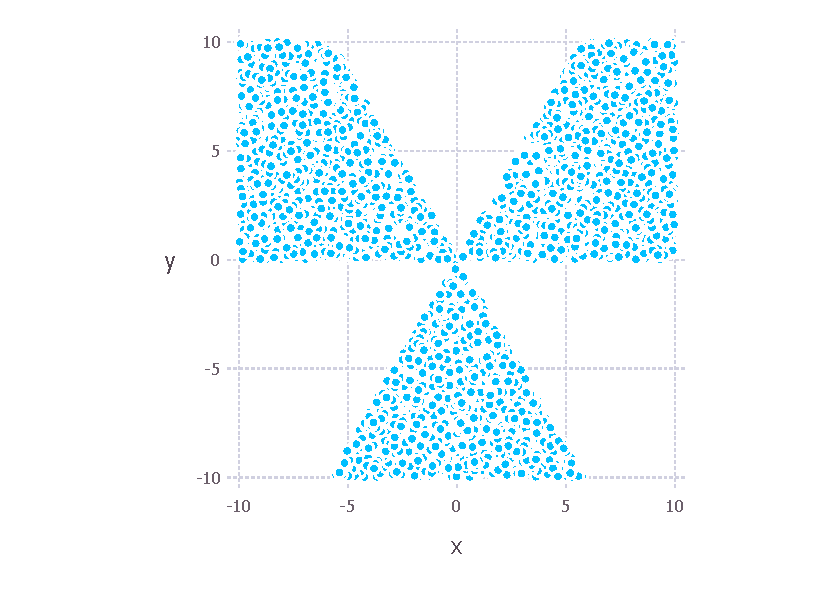
\includegraphics[width=\linewidth]{contourTracingPlot1.pdf}
    \endminipage\hfill
    \minipage{0.32\textwidth}
      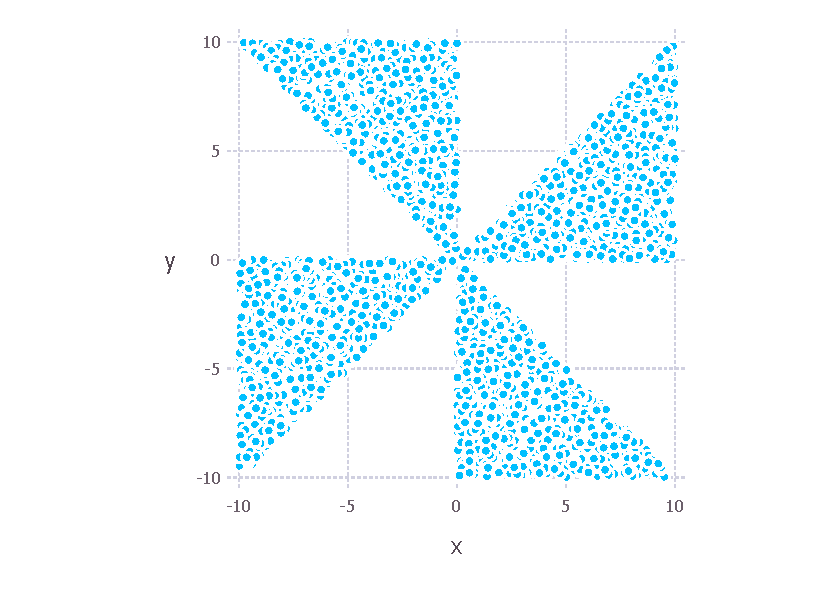
\includegraphics[width=\linewidth]{contourTracingPlot2.pdf}
    \endminipage\hfill
    \minipage{0.32\textwidth}%
      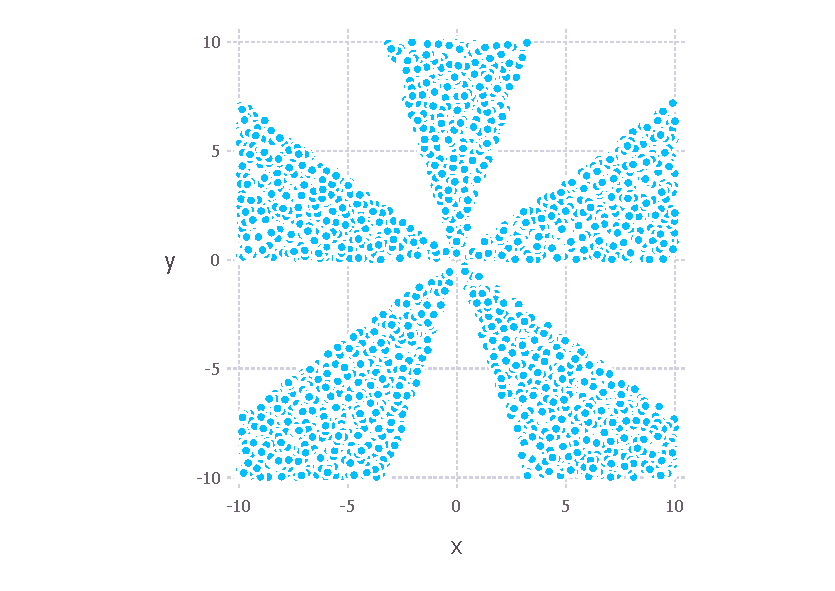
\includegraphics[width=\linewidth]{contourTracingPlot3.pdf}
    \endminipage
    \caption{Simulation of sectors in the domain $\{\lambda\in\C:\,\real(a\lambda^n)>0\}$ by point sampling for $a=-i$ and $n=3, 4, 5$, respectively.}
    \label{fig:contourTracing}
\end{figure}

Now, to find the contour $\Gamma$, suppose we have been given the (finitely many) zeroes of $\Delta(\lambda)$ (we may attempt to write a function to find the zeroes; for now, we assume they are user input). Each sector in the boundary is characterized by the angles of the two rays that mark its boundaries, the starting ray and the ending ray. The contour $\Gamma$ is built from the boundaries of these sectors with possible deformations to include the contours encircling the zeroes. Figure \ref{fig:contourPlot} shows the contour $\Gamma$ of some examples. 
\begin{figure}[htpb!]
    \minipage{0.32\textwidth}
      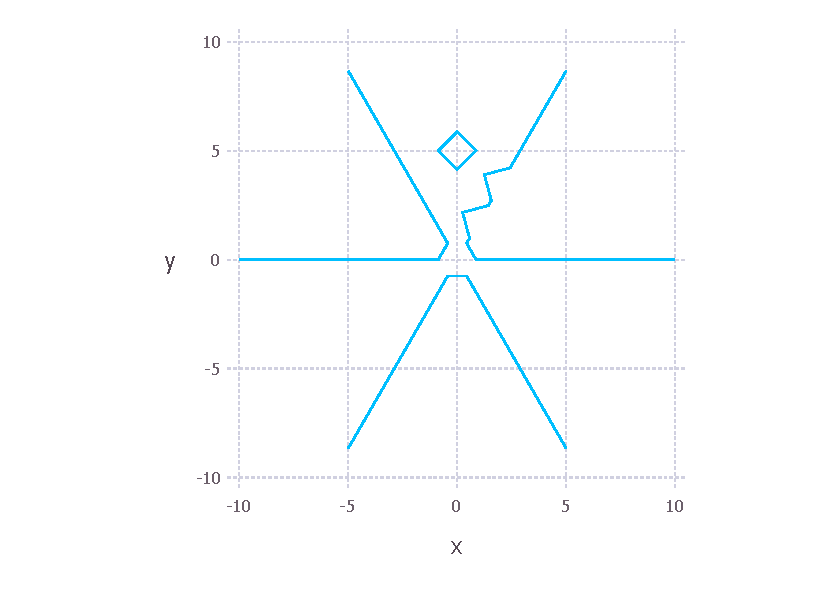
\includegraphics[width=\linewidth]{contourPlot1.pdf}
    \endminipage\hfill
    \minipage{0.32\textwidth}
      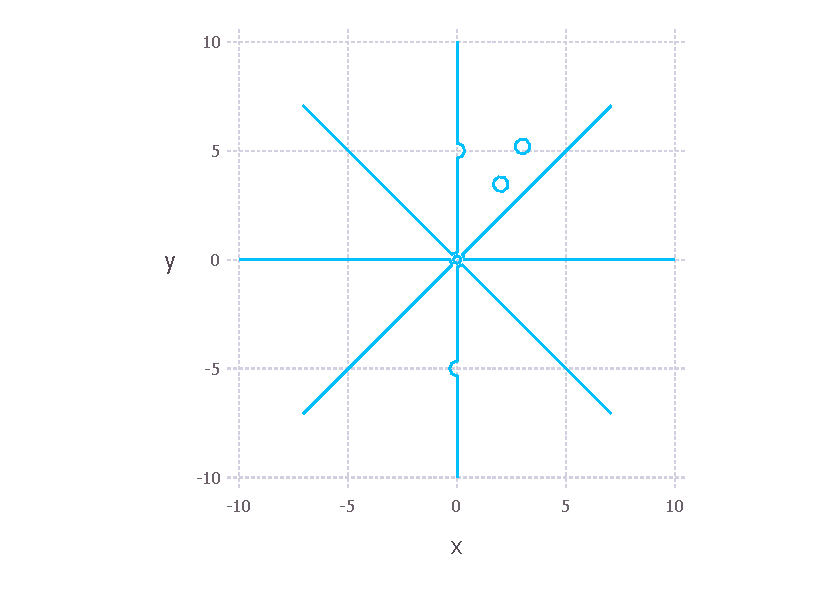
\includegraphics[width=\linewidth]{contourPlot2.pdf}
    \endminipage\hfill
    \minipage{0.32\textwidth}%
      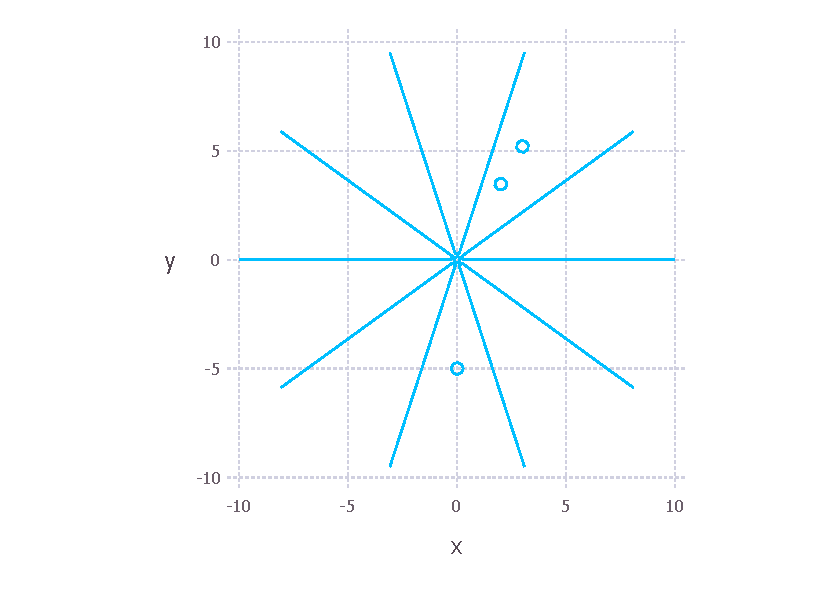
\includegraphics[width=\linewidth]{contourPlot3.pdf}
    \endminipage
    \caption{Characterizing $\Gamma$ for $a=-i$ and $n=3, 4, 5$, respectively, where the zeroes are $1+\sqrt{3}i$, $2+2\sqrt{3}i$, $0+0i$, $0+5i$, $0-5i$.}
    \label{fig:contourPlot}
\end{figure}

For each sector, we initialize its boundary contour by a path consisting of three points, namely a point on the starting ray with distance $d$ from the origin where $d$ is a sufficiently large constant chosen to represent infinity, the origin, and the a point on the ending ray with norm $d$. For each zero, if it is on the boundary of some sector in the domain, we deform its boundary contour to include a small square of radius $\epsilon$ around the zero, where $\epsilon$ is taken to be $1/2$ of the minimum of the pairwise distances between zeroes and the distances between each zero and the starting and ending rays of each sector. If it is exterior to all sectors, we add a square contour to $\Gamma_0^{\pm}$, depending on whether it is in the upper or lower half plane. If it is interior to any sector, we ignore it, since its contribution to the contour integral will be cancelled out. After we have looped through all zeroes in this process, $\Gamma_a$ would contain all sector boundary contours now appropriately deformed, and $\Gamma_0$ would contain all square contours encircling isolated zeroes. Although not reflected in Figure \ref{fig:contourPlot}, care is taken to ensure that the points in $\Gamma$ are listed in the order in which the contour will be integrated over. 

\subsubsection{Chebyshev polynomial approximation}
As pointed out before, we may need to integrate complicated functions and find zeroes of exponential polynomials such as $\Delta(\lambda)$ at future steps in the implementation. Dealing with these complicated functions is difficult, but we may translate it into an easier problem by approximating these complicated functions on given intervals using functions we are more familiar with. To this end, we also implement a method to approximate functions using Chebyshev polynomials in preparation for future work.

The Chebyshev polynomials are given by
\[
    T_n(x) =
\begin{cases}
    \cos(n\cdot \arccos(x))&\quad\mbox{$|x|\leq 1$}\\
    \frac{1}{2}\left((x-\sqrt{x^2-1})^n + (x+\sqrt{x^2-1})^n\right)&\quad\mbox{$|x|>1$}.
\end{cases}    
\]
Given a function $f$ on the interval $[a,b]$, we approximate $f$ using Chebyshev polynomial expansion. The Chebyshev approximation is best on $[-1,1]$. Thus, we scale $[a,b]$ to $[-1,1]$ say via $g:[a,b]\to [-1,1]$, obtain the Chebyshev coefficients $(a_n)_{n=0}^N$ there, and write the approximation of $f$ on $[a,b]$ as
\[f\sim \sum_{n=0}^N a_n\cdot T_n(g(x)),\]
which is a finite sum of Chebyshev polynomials.

\section{Next steps}
With regard to the semester 1 plan in the project proposal, the progress has been on track so far. The immediate next steps would be to finish implementing the Fokas method, organize the implementation into a package, and writing a documentation for the package. These tasks should ideally be completed before the start of semester 2, when emphasis will be put on the second goal of the project as well as preparing project deliverables such as the thesis.


\newpage
\bibliographystyle{unsrt}
% \bibliographystyle{alpha}
\bibliography{C:/Bibtex/Capstone}
\end{document}

